\documentclass[10pt]{beamer}
\usepackage[utf8]{inputenc}
\usepackage[spanish]{babel}

\usetheme{metropolis}

\usepackage{svg}
\usepackage{booktabs}
\usepackage[scale=2]{ccicons}
\usepackage{appendixnumberbeamer}

\usepackage{pgfplots}
\usepgfplotslibrary{dateplot}

\usepackage{xspace}

\newcommand{\themename}{\textbf{\textsc{metropolis}}\xspace}

\title{Introducción a Ethereum}
\date{\today}
\author{@elopio @jeffequivels @rngkll @EdgarBarrantes}
\institute{JáquerEspeis}
\titlegraphic{\hfill
\includegraphics[height=3cm]{images/jaquerespeis.png}}

\begin{document}

\maketitle

\begin{frame}{Tabla de Contenidos}
  \setbeamertemplate{section in toc}[sections numbered]
  \tableofcontents[hideallsubsections]
\end{frame}

\section{Introducción}

\begin{frame}{¿Qué es el dinero?}
  
\end{frame}

\begin{frame}{¿Qué es el dinero?}

  (Esta diapositiva fue dejada en blanco por fines dramáticos)
  
\end{frame}

\begin{frame}{Generales Bizantinos}

  \begin{center}
    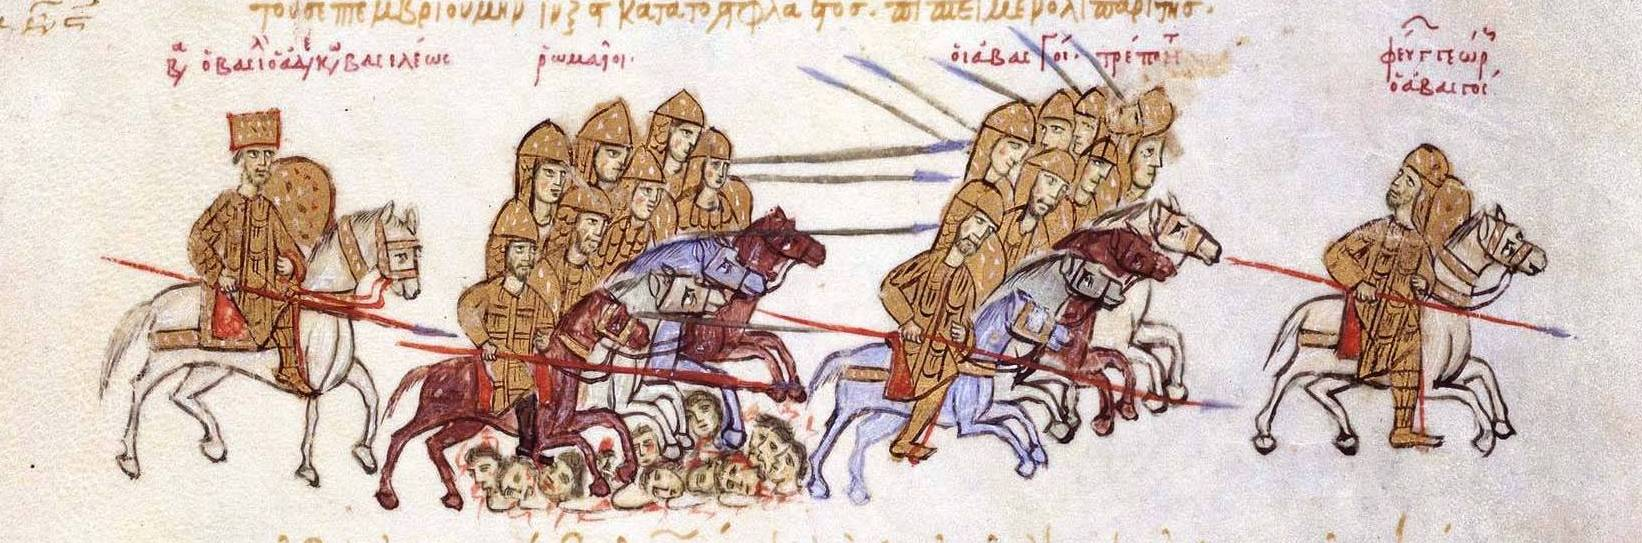
\includegraphics[height=3.5cm]{images/generales-bizantinos.jpg}
    \\ (imagen tomada de \href{https://commons.wikimedia.org/w/index.php?title=File:Skylitzes._Basil_II_vs_Georgians_cropped.jpg&oldid=181584464}{Wikipedia})
  \end{center}
  
\end{frame}

\begin{frame}{Generales Bizantinos}

  \begin{itemize}
    \item ¿Atacamos o huimos?
    \item Un ataque a medias va a ser desastrozo, necesitamos consenso.
    \item ¿En quién podemos confiar?
  \end{itemize}
  
\end{frame}

\begin{frame}{Satoshi}

  \begin{center}
    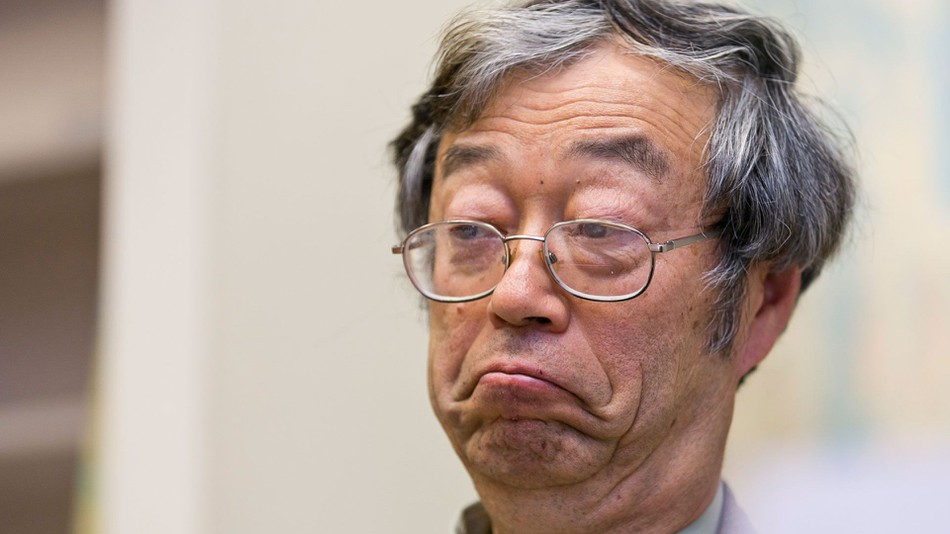
\includegraphics[height=3.5cm]{images/satoshi.jpg}
    \\ Hold my beer!
    \\ (imagen tomada sin permiso de \href{https://mashable.com/2014/03/07/dorian-nakamoto-bitcoin}{Mashable})
  \end{center}
  
\end{frame}

\begin{frame}{Bitcoin}

  \begin{itemize}
    \item Un libro mayor, pero distribuido.
    \item Prueba de trabajo para llegar a consenso.
    \item Algoritmo de hash.
    \item Premio de minado para incentivar buen comportamiento.
    \item Lenguaje sencillo para transacciones
  \end{itemize}
  
\end{frame}

\section{Ethereum}

\begin{frame}{Ethereum}

  \begin{itemize}
    \item Turing completo.
    \item No es eficiente, todos los nodos ejecutan las mismas instrucciones.
    \item Transparente.
    \item Múltiples verificaciones.
    \item Inmutable.
  \end{itemize}
  
\end{frame}

\begin{frame}{Ethash}

  \begin{itemize}
    \item Hay una semilla.
    \item De la semilla se calcula una caché pseudoaleatoria de 16 MB.
    \item De la caché se genera un conjunto de datos de 1 GB.
    \item Minar es tomar secciones aleatorias del conjunto de datos, y hacerles un hash.
    \item Está limitado por memoria, porque la mayoría del trabajo está en leer los datos.
    \item La verificación se hace sólo con la caché.
    \item Es una solución temporal, durante la investigación de Prueba de participación.
  \end{itemize}
  
\end{frame}

\section{Cadena de bloques}

\begin{frame}{Bloque}
	\begin{itemize}
		\item Un grupo de transacciones.
		\item Con una marca de tiempo.
		\item La dirección del bloque anterior.
		\item Y la prueba de trabajo que valida todas las transacciones.
	\end{itemize}
\end{frame}

\begin{frame}{Transacciones}
	\begin{itemize}
		\item Mensajes firmados por una cuenta.
		\item Se transmiten a través de la red de Ethereum.
		\item Se guardan en la cadena de bloques.
		\item Solicitud de cambio de estado o de ejecución de un contrato.
		\item Son atómicas.
	\end{itemize}
\end{frame}

\begin{frame}{Árbol Merkle}
  \begin{itemize}
    \item Estructura de datos autenticada con criptografía.
    \item Almacena parejas (clave, valor).
    \item Totalmente deterministico, si dos árboles contienen los mismos datos, tienen el mismo hash raíz.
    \item Eficiente para inserciones, búsquedas y borrados.
  \end{itemize}
\end{frame}

\begin{frame}{De vuelta a los bloques}
  \begin{itemize}
    \item Cada bloque tiene tres árboles.
    \item Estado: dirección, balance y datos de contratos.
    \item Transacciones: solicitudes de transacciones.
    \item Recibos: resultados de transacciones.
  \end{itemize}
\end{frame}

\section{Direcciones}

\begin{frame}{clave pública, clave privada}
  \begin{itemize}
    \item Se basan en funciones que son fáciles de calcular en una dirección, pero muy difíciles de calcular en la dirección contraria.
     \item Multiplicar dos números primos grandes es fácil; pero dado el producto, es muy dificil encontrar los dos números.
    \item Encontrar la clave privada dado una clave pública es tan dificil como probar todos los posibles valores en un ataque de fuerza bruta.
  \end{itemize}
\end{frame}

\begin{frame}{clave pública, clave privada}
  \begin{itemize}
    \item La clave privada se utiliza para generar mensajes firmados.
    \item La clave pública se utiliza para validar las firmas sin revelar la clave privada.
    \item La clave pública se genera a partir de una clave privada.
    \item Las direcciones se generan a partir de una clave pública.
    \item Las transacciones requieren una firma válida.
  \end{itemize}
\end{frame}

\begin{frame}{Criptografía de curvas elípticas}
  \begin{center}
    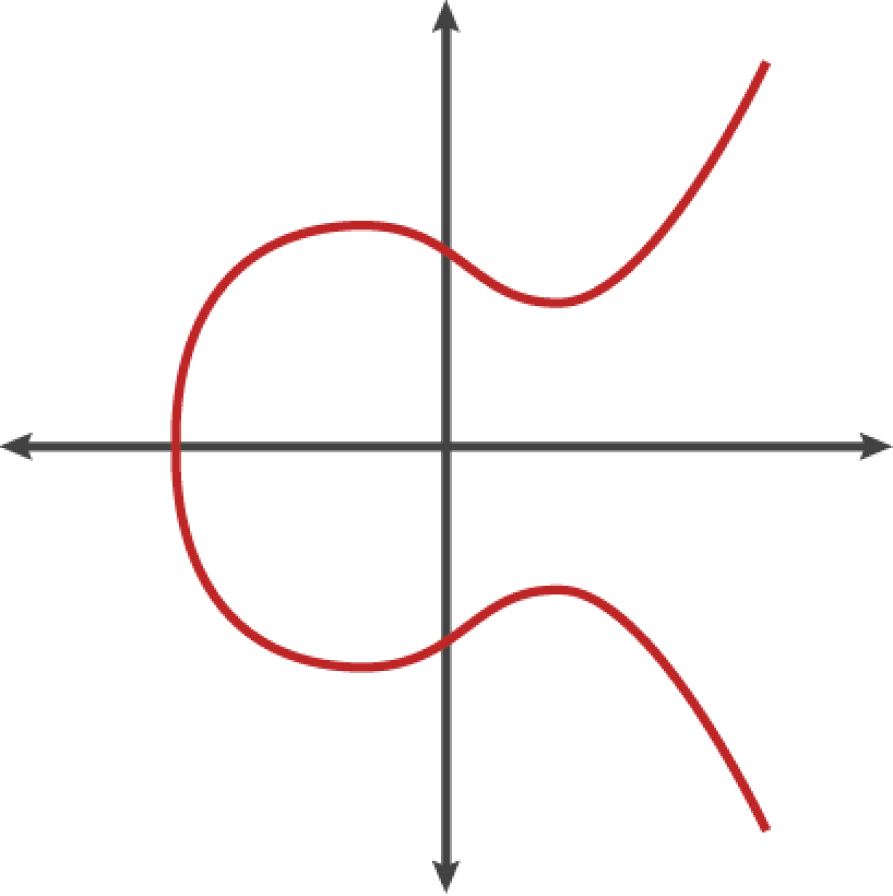
\includegraphics[height=4cm]{images/simple_elliptic_curve.png}
    \\ (imagen tomada de \href{https://github.com/ethereumbook/ethereumbook}{Mastering Ethereum})
  \end{center}
\end{frame}

\begin{frame}{Criptografía de curvas elípticas}
  \begin{itemize}
    \item La clave privada es un número aleatorio entre $1$ y $1.158 \times 10^{77} - 1$, algo como: \begin{tiny}$f8f8a2f43c8376ccb0871305060d7b27b0554d2cc72bccf41b2705608452f315$\end{tiny}
    \item Suma: dados dos puntos P1 y P2 en la curva, hay un tercer punto P3 = P1 + P2, también en la curva.
    \item Mutiplicación: aplicar la suma múltiples veces.
    \item Para generar la clave pública: $pub = priv \times generador$
  \end{itemize}
\end{frame}

\begin{frame}{Monederos}
  \begin{itemize}
    \item Las claves no se almacenan en la blockchain.
    \item No contienen dinero, permiten utilizar el dinero.
    \item Software que facilita firmar transacciones.
  \end{itemize}
\end{frame}

\section{Contratos inteligentes}

\begin{frame}[fragile]{Solidity}
  \begin{itemize}
    \item Contratos: programas inmutables que ejecutan de forma determinística.
    \item Solidity: un lenguaje para escribir contratos inteligentes.
  \end{itemize}
  \begin{verbatim}
    contract Faucet {
      function withdraw(uint withdraw_amount) public {
        msg.sender.transfer(withdraw_amount);
      }
    }
  \end{verbatim}
\end{frame}

\begin{frame}[fragile]{OpenZeppelin}
  Un framework para construir contratos seguros.
  \\ https://github.com/OpenZeppelin/openzeppelin-solidity
  \begin{verbatim}
contract SampleCrowdsale 
    is CappedCrowdsale, RefundableCrowdsale, MintedCrowdsale {
  constructor(
    uint256 _openingTime, uint256 _closingTime,
    uint256 _rate, address _wallet, uint256 _cap, uint256 _goal,
    MintableToken _token
  )
    public
    Crowdsale(_rate, _wallet, _token)
    CappedCrowdsale(_cap)
    TimedCrowdsale(_openingTime, _closingTime)
    RefundableCrowdsale(_goal)
  {
    require(_goal <= _cap);
  }
}
  \end{verbatim}
\end{frame}

\begin{frame}{Seguridad}
  \begin{itemize}
    \item Los contratos reciben y envían ether, y otras representaciones con valor económico.
    \item Una vulnerabilidad en el código puede significar perder mucho dinero.
    \item Reusar código, escribir código simple y claro, fallar lo más pronto posible, escribir pruebas.
    \item Agregar mecanismos de emergencia, aprender las particularidades del lenguaje y la plataforma, aprender de las vulnerabilidades encontradas.
  \end{itemize}
\end{frame}

\section{Ether y gas}

\begin{frame}{Unidades}
  \begin{itemize}
    \item La unidad básica es el wei.
    \item 1 ether es 1 quintillon de wei o $1 \times 10^{18}$ o $1,000,000,000,000,000,000$
    \item 1 ether hoy vale cerca de \$700.
  \end{itemize}
\end{frame}

\begin{frame}{Gas}
  \begin{itemize}
    \item Unidad para medir cuánto poder computacional requiere un programa.
    \item Cada operación cuesta cierta cantidad de gas.
    \item Sumar dos números cuesta 3 gas.
    \item Enviar una transacción cuesta 21000 gas.
  \end{itemize}
\end{frame}

\begin{frame}{Gas}
  \begin{itemize}
    \item Quien inicia una transacción establece el precio al que va a pagar cada unidad de gas, en ether.
    \item Y establece el límite de gas que está dispuesta a pagar.
    \item Se le paga a quien mina la transacción.
  \end{itemize}
\end{frame}

\section{EVM}

\begin{frame}{EVM}
  \begin{itemize}
    \item Las instrucciones de los contratos se ejecutan en una máquina virtual.
    \item Funciona dentro de una caja de arena, completamente aislada de la red, el sistema de archivo y otros procesos de la máquina que la ejecuta.
    \item Cada nodo en la red de ethereum ejecuta una implementación de la EVM.
    \item Por ejemplo: parity, geth.
    \item Los nodos ejecutan los contratos en la EVM y llegan a un consenso sobre el resultado.
  \end{itemize}
\end{frame}

\section{Taller}

\begin{frame}{CryptoZombies}
  https://cryptozombies.io/es/
\end{frame}

\begin{frame}{¿Cómo hacer un ICO}
  https://zpl.in/howto-ico
\end{frame}

\begin{frame}{Ethernaut}
  https://zpl.in/ethernaut
\end{frame}

\begin{frame}{Créditos}

  Esta presentación se hizo con los programas libres \href{https://www.latex-project.org/}{LaTeX} y \href{https://www.sharelatex.com/}{ShareLaTeX}.

  El código para el tema gráfico lo hizo \href{https://github.com/matze/mtheme}{Matthias Vogelgesang}.
  
  Esta presentación está liberada con la licencia \href{http://creativecommons.org/licenses/by-sa/4.0/}{Creative Commons
  Attribution-ShareAlike 4.0 International}.

  \begin{center}\ccbysa\end{center}

\end{frame}

\end{document}
